%%%==============================================================================
% WinEdt pragmas
% !Mode:: "TeX:EN"
% Default Compile engines:
% !TEX program = pdflatex
% !PDFTeXify ext =  --enable-etex  --restrict-write18
% !PDFLaTeX ext  =  --enable-etex  --restrict-write18
% !BIB program = none

\documentclass[a4paper,10pt]{article}
\usepackage{a4wide}

\usepackage[T1]{fontenc}
\usepackage[utf8]{inputenc}
\usepackage{xcolor}
\usepackage{codedescribe}

\usepackage[american,siunitx,cuteinductors,smartlabels,arrowmos,EFvoltages,betterproportions]{circuitikz}
\usetikzlibrary{math}

\usepackage{tikzdotncross}
\usepackage{tikzquads}

\showcoordstrue

\begin{document}

All default Quadripoles and Thevenin/Norton.

\begin{codestore}[DemoA]
\resizebox{\textwidth}{!}{
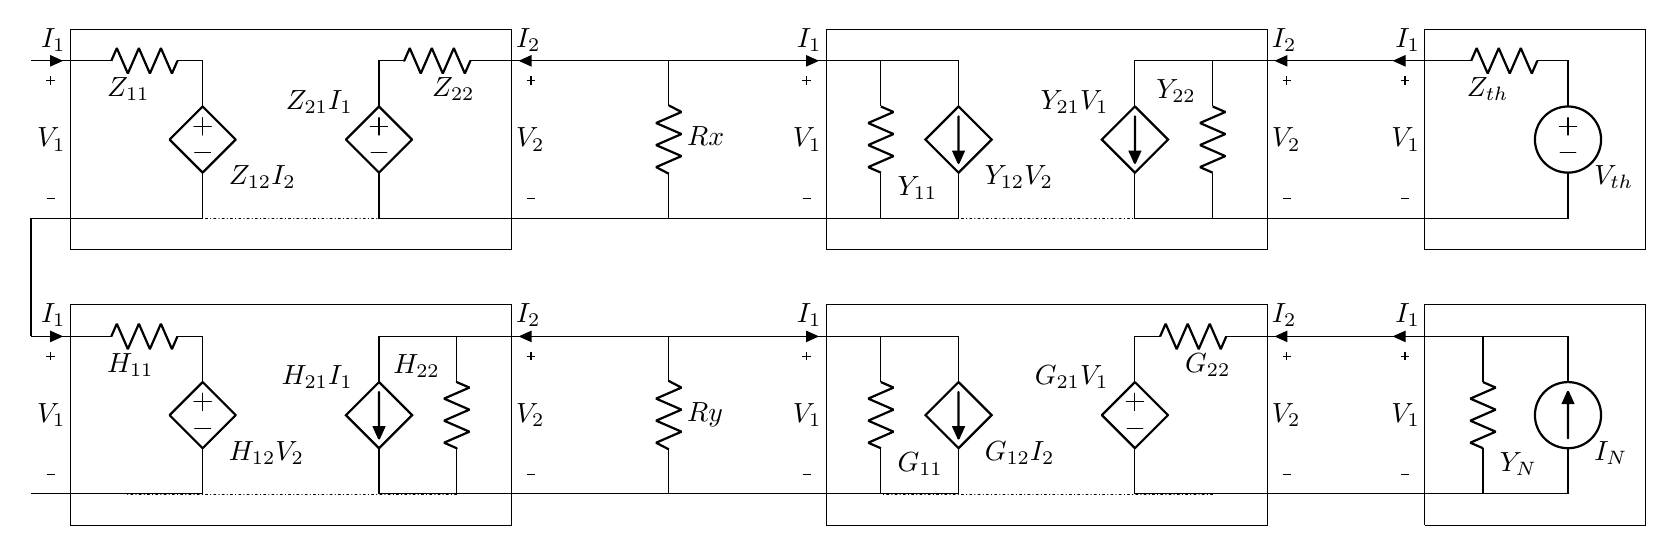
\begin{tikzpicture}
  \draw (0,0) \ncoord(ref) node[Quad Z,anchor=1+](Qz1){}
    (Qz1.2+) -- ++(1.5,0) \ncoord(X) -- ++(1.5,0) node[Quad Y,anchor=1+](Qy1){}
    (Qy1.2+) -- ++(1,0) node[Thevenin,anchor=1+](th1){}
    (Qz1.1-) -- ++(0,-1.5) node[Quad H,anchor=1+](Qh1){}
    (Qh1.2+) -- ++(1.5,0) \ncoord(Y) -- ++(1.5,0) node[Quad G,anchor=1+](Qg1){}
    (Qg1.2+) -- ++(1,0) node[Norton,anchor=1+](nr1){}
    (Qz1.2-) -- (Qy1.1-) (Qy1.2-) -- (th1.1-)
    (Qh1.2-) -- (Qg1.1-) (Qg1.2-) -- (nr1.1-)
    ;
  \draw (X) to[R=$Rx$] (X |- Qz1.2-)
        (Y) to[R=$Ry$] (Y |- Qh1.2-) 
        ;
\end{tikzpicture}
}
\end{codestore}

\tsdemo*[emph={draw,node,coord},emph2={x,y,fit,to,outer,inner,round,control,sources,european,alt},emph3={Quad,Black,Box},basicstyle={\scriptsize\ttfamily},numbers=left]{DemoA}

~


The same demo but with all parameter $11$ and $22$ zeroed, and changing the ``control sources''

\begin{codestore}[DemoB]
\resizebox{\textwidth}{!}{
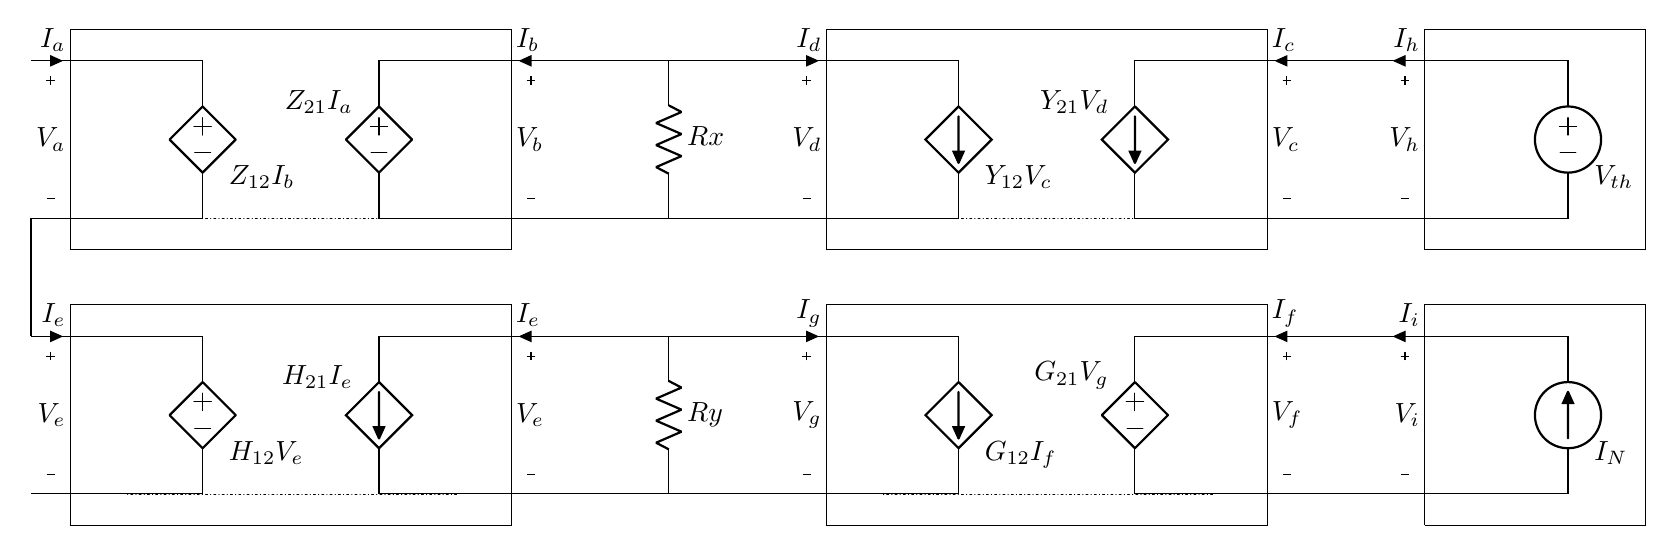
\begin{tikzpicture}
  \draw (0,0) \ncoord(ref) node[Quad Z,anchor=1+,Z11=0,Z22=0,I1=$I_a$,V1=$V_a$,I2=$I_b$,V2=$V_b$](Qz1){}
    (Qz1.2+) -- ++(1.5,0) \ncoord(X) -- ++(1.5,0) node[Quad Y,anchor=1+,Y11=0,Y22=0,I1=$I_d$,V1=$V_d$,I2=$I_c$,V2=$V_c$](Qy1){}
    (Qy1.2+) -- ++(1,0) node[Thevenin,anchor=1+,Zth=0,I1=$I_h$,V1=$V_h$](th1){}
    (Qz1.1-) -- ++(0,-1.5) node[Quad H,anchor=1+,H11=0,H22=0,I1=$I_e$,V1=$V_e$,I2=$I_e$,V2=$V_e$](Qh1){}
    (Qh1.2+) -- ++(1.5,0) \ncoord(Y) -- ++(1.5,0) node[Quad G,anchor=1+,G11=0,G22=0,I1=$I_g$,V1=$V_g$,I2=$I_f$,V2=$V_f$](Qg1){}
    (Qg1.2+) -- ++(1,0) node[Norton,anchor=1+,Yn=0,I1=$I_i$,V1=$V_i$](nr1){}
    (Qz1.2-) -- (Qy1.1-) (Qy1.2-) -- (th1.1-)
    (Qh1.2-) -- (Qg1.1-) (Qg1.2-) -- (nr1.1-)
    ;
  \draw (X) to[R=$Rx$] (X |- Qz1.2-)
        (Y) to[R=$Ry$] (Y |- Qh1.2-) 
        ;
\end{tikzpicture}
}
\end{codestore}

\tsdemo*[emph={draw,node,coord},emph2={x,y,fit,to,outer,inner,round,control,sources,european,alt},emph3={Quad,Black,Box},basicstyle={\scriptsize\ttfamily},numbers=left]{DemoB}
~


Now with the $12$ and $21$ parameters zeroed, normal form:

\begin{codestore}[DemoC]
\resizebox{\textwidth}{!}{
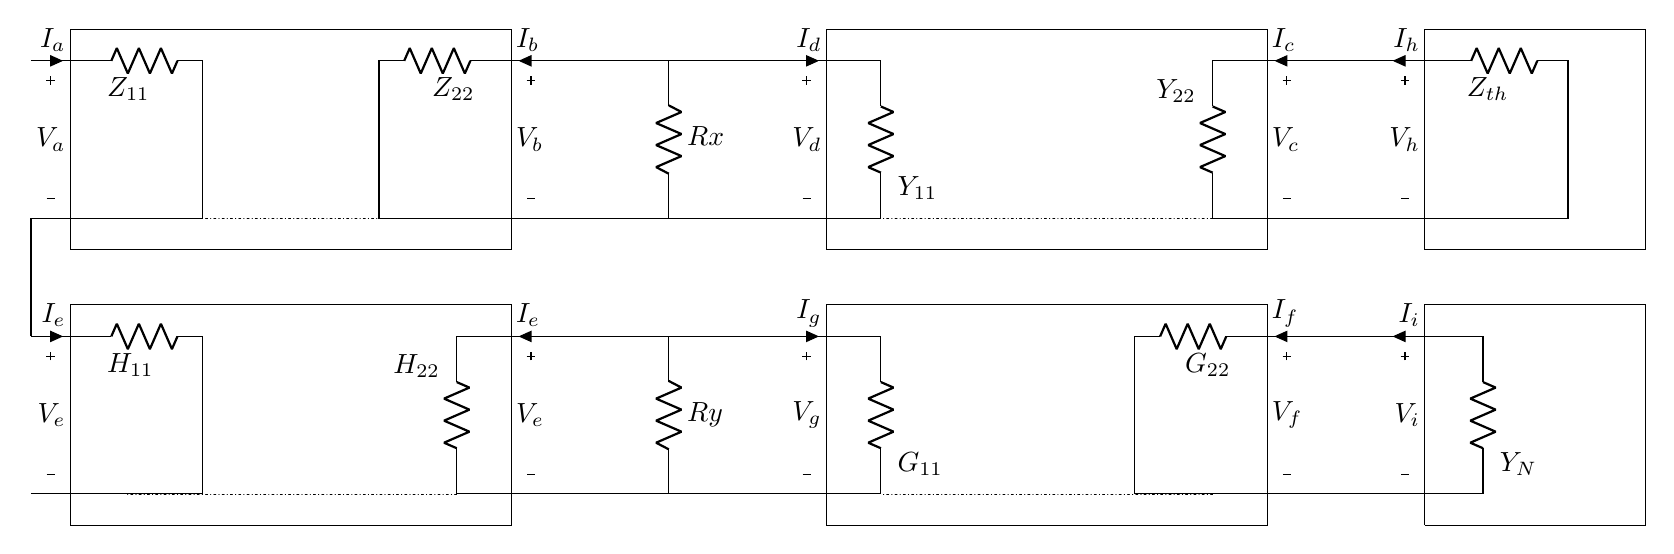
\begin{tikzpicture}
  \draw (0,0) \ncoord(ref) node[Quad Z,anchor=1+,Z12=0,Z21=0,I1=$I_a$,V1=$V_a$,I2=$I_b$,V2=$V_b$](Qz1){}
    (Qz1.2+) -- ++(1.5,0) \ncoord(X) -- ++(1.5,0) node[Quad Y,anchor=1+,Y12=0,Y21=0,I1=$I_d$,V1=$V_d$,I2=$I_c$,V2=$V_c$](Qy1){}
    (Qy1.2+) -- ++(1,0) node[Thevenin,anchor=1+,Vth=0,I1=$I_h$,V1=$V_h$](th1){}
    (Qz1.1-) -- ++(0,-1.5) node[Quad H,anchor=1+,H12=0,H21=0,I1=$I_e$,V1=$V_e$,I2=$I_e$,V2=$V_e$](Qh1){}
    (Qh1.2+) -- ++(1.5,0) \ncoord(Y) -- ++(1.5,0) node[Quad G,anchor=1+,G12=0,G21=0,I1=$I_g$,V1=$V_g$,I2=$I_f$,V2=$V_f$](Qg1){}
    (Qg1.2+) -- ++(1,0) node[Norton,anchor=1+,In=0,I1=$I_i$,V1=$V_i$](nr1){}
    (Qz1.2-) -- (Qy1.1-) (Qy1.2-) -- (th1.1-)
    (Qh1.2-) -- (Qg1.1-) (Qg1.2-) -- (nr1.1-)
    ;
  \draw (X) to[R=$Rx$] (X |- Qz1.2-)
        (Y) to[R=$Ry$] (Y |- Qh1.2-) 
        ;
\end{tikzpicture}
}
\end{codestore}

\tsdemo*[emph={draw,node,coord},emph2={x,y,fit,to,outer,inner,round,control,sources,european,alt},emph3={Quad,Black,Box},basicstyle={\scriptsize\ttfamily},numbers=left]{DemoC}

~

Same as last one, but with an alternate form:

\begin{codestore}[DemoC]
\resizebox{\textwidth}{!}{
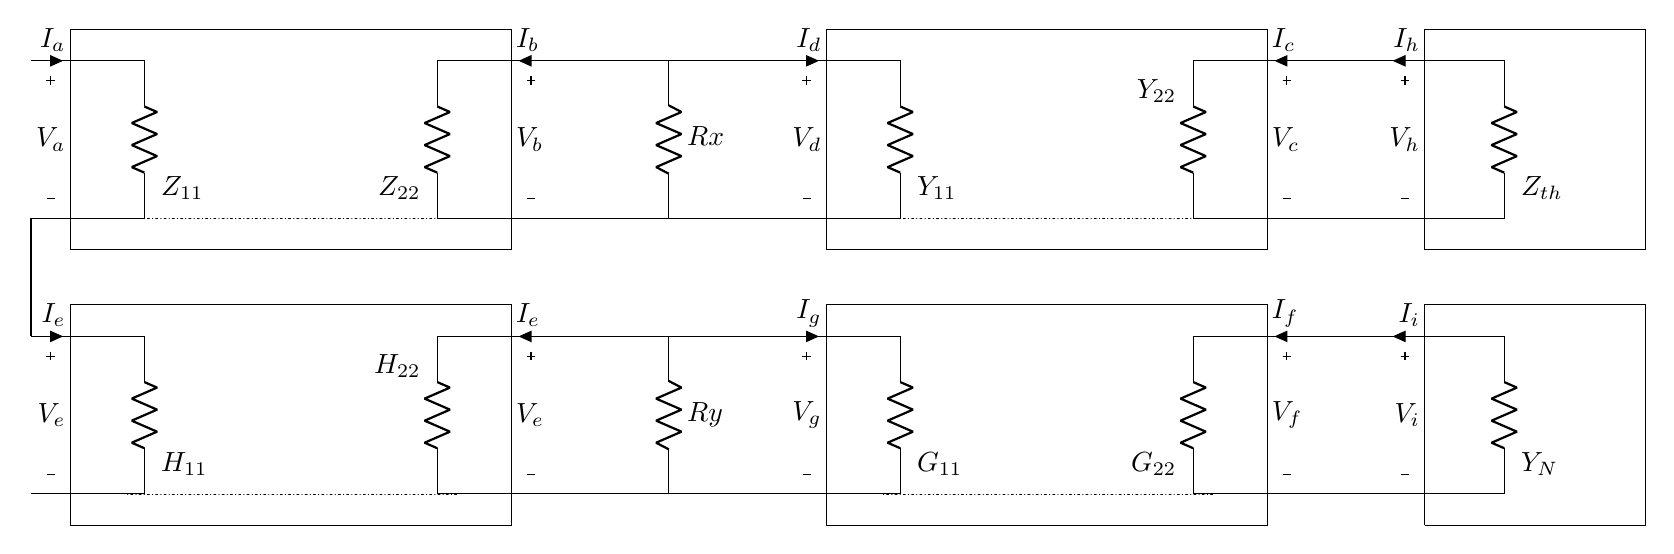
\begin{tikzpicture}
  \draw (0,0) \ncoord(ref) node[Quad Z,alt,anchor=1+,Z12=0,Z21=0,I1=$I_a$,V1=$V_a$,I2=$I_b$,V2=$V_b$](Qz1){}
    (Qz1.2+) -- ++(1.5,0) \ncoord(X) -- ++(1.5,0) node[Quad Y,alt,anchor=1+,Y12=0,Y21=0,I1=$I_d$,V1=$V_d$,I2=$I_c$,V2=$V_c$](Qy1){}
    (Qy1.2+) -- ++(1,0) node[Thevenin,alt,anchor=1+,Vth=0,I1=$I_h$,V1=$V_h$](th1){}
    (Qz1.1-) -- ++(0,-1.5) node[Quad H,alt,anchor=1+,H12=0,H21=0,I1=$I_e$,V1=$V_e$,I2=$I_e$,V2=$V_e$](Qh1){}
    (Qh1.2+) -- ++(1.5,0) \ncoord(Y) -- ++(1.5,0) node[Quad G,alt,anchor=1+,G12=0,G21=0,I1=$I_g$,V1=$V_g$,I2=$I_f$,V2=$V_f$](Qg1){}
    (Qg1.2+) -- ++(1,0) node[Norton,alt,anchor=1+,In=0,I1=$I_i$,V1=$V_i$](nr1){}
    (Qz1.2-) -- (Qy1.1-) (Qy1.2-) -- (th1.1-)
    (Qh1.2-) -- (Qg1.1-) (Qg1.2-) -- (nr1.1-)
    ;
  \draw (X) to[R=$Rx$] (X |- Qz1.2-)
        (Y) to[R=$Ry$] (Y |- Qh1.2-) 
        ;
\end{tikzpicture}
}
\end{codestore}

\tsdemo*[emph={draw,node,coord},emph2={x,y,fit,to,outer,inner,round,control,sources,european,alt},emph3={Quad,Black,Box},basicstyle={\scriptsize\ttfamily},numbers=left]{DemoC}

~


And a final one, no zeroed parameters, but all ``non default'', some impedances as zig-zag, others as generic, per quadripole



\begin{codestore}[DemoD]
\resizebox{\textwidth}{!}{
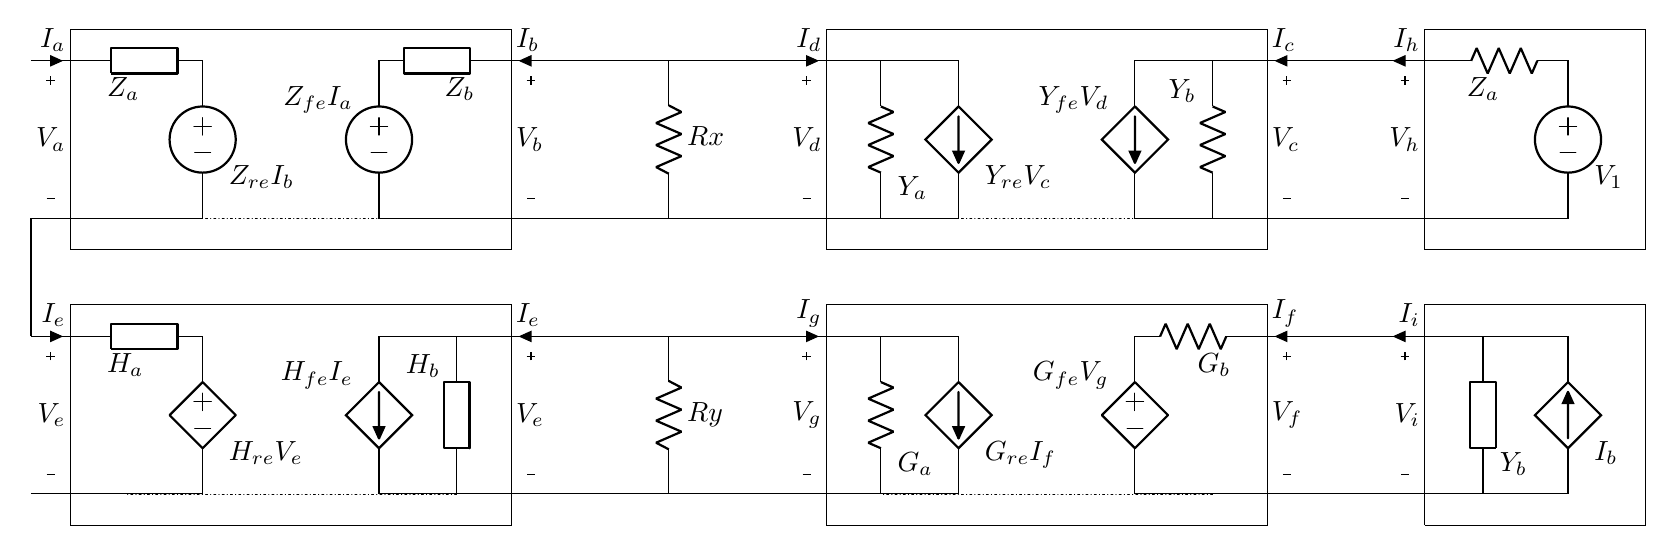
\begin{tikzpicture}
  \draw (0,0) \ncoord(ref) node[Quad Z,alt,round sources,european,anchor=1+,Z11=$Z_a$,Z22=$Z_b$,Z12=$Z_{re}$,Z21=$Z_{fe}$,I1=$I_a$,V1=$V_a$,I2=$I_b$,V2=$V_b$](Qz1){}
    (Qz1.2+) -- ++(1.5,0) \ncoord(X) -- ++(1.5,0) node[Quad Y,alt,anchor=1+,Y11=$Y_a$,Y22=$Y_b$,Y12=$Y_{re}$,Y21=$Y_{fe}$,I1=$I_d$,V1=$V_d$,I2=$I_c$,V2=$V_c$](Qy1){}
    (Qy1.2+) -- ++(1,0) node[Thevenin,alt,anchor=1+,Vth=$V_1$,Zth=$Z_a$,I1=$I_h$,V1=$V_h$](th1){}
    (Qz1.1-) -- ++(0,-1.5) node[Quad H,european,alt,anchor=1+,H11=$H_a$,H22=$H_b$,H12=$H_{re}$,H21=$H_{fe}$,I1=$I_e$,V1=$V_e$,I2=$I_e$,V2=$V_e$](Qh1){}
    (Qh1.2+) -- ++(1.5,0) \ncoord(Y) -- ++(1.5,0) node[Quad G,alt,anchor=1+,G11=$G_a$,G22=$G_b$,G12=$G_{re}$,G21=$G_{fe}$,I1=$I_g$,V1=$V_g$,I2=$I_f$,V2=$V_f$](Qg1){}
    (Qg1.2+) -- ++(1,0) node[Norton,alt,control sources,european,anchor=1+,In=$I_b$,Yn=$Y_b$,I1=$I_i$,V1=$V_i$](nr1){}
    (Qz1.2-) -- (Qy1.1-) (Qy1.2-) -- (th1.1-)
    (Qh1.2-) -- (Qg1.1-) (Qg1.2-) -- (nr1.1-)
    ;
  \draw (X) to[R=$Rx$] (X |- Qz1.2-)
        (Y) to[R=$Ry$] (Y |- Qh1.2-) 
        ;
\end{tikzpicture}
}
\end{codestore}

\tsdemo*[emph={draw,node,coord},emph2={x,y,fit,to,outer,inner,round,control,sources,european,alt},emph3={Quad,Black,Box},basicstyle={\scriptsize\ttfamily},numbers=left]{DemoD}


\end{document}
